\documentclass[11pt,singlecolumn]{scrartcl}
\usepackage[bachelorthesis]{systems-cover}
\usepackage{amsmath,amssymb,amstext}
\usepackage[utf8]{inputenc}
\usepackage[english]{babel}
\usepackage{fancyhdr}
\usepackage{graphicx}
\usepackage[capposition=bottom]{floatrow}
\pagestyle{fancy}
\fancyhf{}
\fancyhead[LE,RO]{Druid vs. AIM}
\fancyhead[RE,LO]{Lukas Striebel}

\fancyfoot[RE,lO]{Bachelor Thesis}
\fancyfoot[LE,RO]{\thepage}

\renewcommand{\headrulewidth}{2pt}
\renewcommand{\footrulewidth}{1pt}

\covernum{132 b}
\covertitle{Druid vs. AIM}
\coverauthor{Lukas Striebel}
\coverdate{09.02.2015 - 09.07.2015}
\coversupervisedby{Prof.\ Donald Kossmann, Lucas Braun, Renato Marroquin}

\begin{document}

\hspace{60mm}
\begin{center}
 \textbf{Abstract} \end{center}


In today's society, data is arguably one of the most valuable goods. In recent years, many related research fields have  spawned: data mining, protecting data, storing data, just to name a few. Dealing with huge amount of data is without doubt essential for any company. In this thesis two different data stores, AIM and Druid, are compared aginst each other. The thesis further explores how these two system could be used together in order to support each other.


\clearpage
\tableofcontents
\clearpage
\section{Introduction}
\subsection{Motivation}
To follow

\subsection{Thesis Structure}
The remainder is structured as follows. In Section 2 The Druid and AIM systems are introduced and the benchmark is explained. Section 3 contains the different approaches, both successful and unsuccessful, on how to run this benchmark on Druid. The obtained results are discussed in section 4. Section 5 concludes the thesis.
\clearpage

\section{Background}
\subsection{The AIM Architecture}
The AIM system \cite{aim} is currently being developped at ETH by various people. It is designed for storing large amounts of data as well as dealing with synchronous updates and queries. A possible usecase would be a telecommunication company, where the updates can be seen as calls between customers and the queries as retrieving certain statistics of said customers, e.g. average call duration, numbers of calls this weekand so on.\\\\
The core idea  behind AIM is to have two seperate parts, the SEP and the RTA. Both parts operate on a large amount of data, called the \textit{Analytics Matrix}, which can be imagined as a very large and wide table. The \textit{Stream Event Processing} (SEP) receives updates and modifies the Analytics Matrix accordingly. Due to its size, the Analytics Matrix is usually not stored on a single machine, but instead distributed amongst multiple data store nodes. The \textit{Real-Time Analytics Processing} (RTA) is responsible for processing the queries and gathering the partial results form the various distributed data store nodes.

\begin{figure}[h]
\includegraphics[scale=0.55]{aim.jpg}
\caption{The AIM architecture, graphic taken from \cite{aim}}
\end{figure}

\clearpage

\subsection{The Druid Architecture}
Developed by Metamarkets Inc., the druid system  \cite{druid} is built on four types of different nodes, each of them fullfilling one of these tasks: ingesting, storing, querying and coordinating. The Overdlord resp. the Realtime Node is responsible for the data ingression. The difference between them is that the Realtime node is used incase of a continous data stream, e.g. Amazon sales, whereas the Overlord is used whenever the data to be ingested is already known, as is it the case in the AIM benchmark.\\
The Historical node saves the ingested data segments on Deep Storage, which can be the hard disk, Amazon S3 or whatever specified.\\
The Broker node directs incoming queries to the corresponding Historical node.\\
The Coordinator in combination with Zookeeper \cite{zoo} manages the interactions between the different Nodes.\\


\begin{figure}[h]
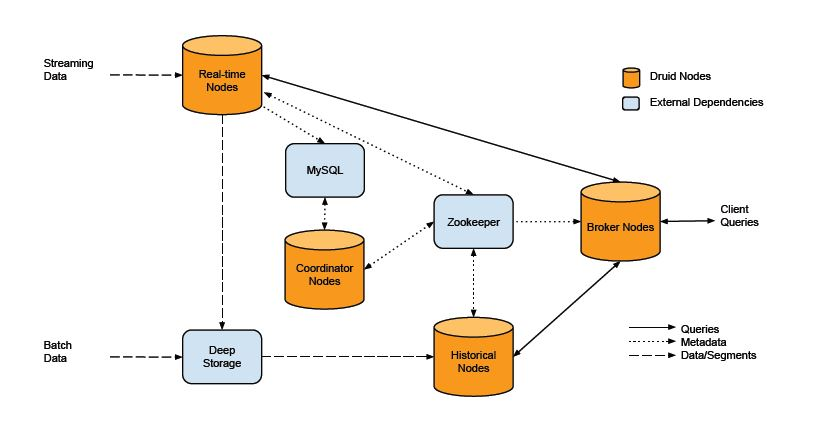
\includegraphics[scale=0.7]{druid.jpg}
\caption{The Druid architecture, graphic taken from \cite{druid}}
\end{figure}

There are a number of extensions compatible with druid, most notably hadoop \cite{hadoop}, which will be used later on in this thesis. Hadoop on its own is already a formidable data store, however in our case we will only use it to replace the Overlord node. As stated by the developers and verified by personal experience, the Overlord works efficient only as long as size of the data file is below 1 GB. After crossing this threshold, performance drops significantly. We therefore used a single node hadoop cluster for the ingestion of larger files.
\\[1cm]
Druid is opensource and currently available at \cite{druidon}.

\clearpage

\subsection{The Benchmark}
The original benchmark consist of two parts, one for the RTA and one for the SEP. In this benchmark the Analytics Matrix contained a total of ten million subscribers. Each customer possesed 42 unique attributes such as number of calls or longest call duration. These 42 attributes were duplicated 13 times in order to create a more realistic environment. This resulted in a total amount of 546 attributes per subscriber. In the SEP part the time it took to apply three million updates to the Analytics Matrix was measured. In the RTA part the performance for answering seven different queries, featuring various Joins and Aggregations, was measured. 
\clearpage

\section{Methods}

\subsection{First Attempts}
In our first attempts we tried to implement exactly the same AIM benchmark on Druid. This meant that Druid had to store only one row for each customer, which contains various static attributes such as subscriberid, postal code etc., as well as the entire 546 aggregations, resulting in a very wide table. However, it also yields the benfit of having a table of constant size, rather than an evergrowing one. Approaching the benchmark this way greatly simplified the RTA part. Since Druid doesn't speak SQL, the only thing to do was to translate the original 7 query into a format that Druid was able to understand.\\\\
However, it soon became clear that updating existing data in Druid is quite difficult, since Druid doesn't feature any kind of native updating functionality. Instead it is suggested to simply ingest a new, more up-to-date record, which will overwrite the existing one. Therefore the only possible way to execute an update in the sense of the SEP benchmark would be to send a query to retrieve the old record, manually update it and then reingest that data. Unsurprisingly, this approach performed very poorly timewise. This posed an insurmountable problem, and we failed to come up with a solution. However, we decided to take a different path.    


\subsection{Rethinking the benchmark}
As AIM lacks a reliable recovery system, we decide to instead test whether Druid could be used make a suitable backup for AIM. This meant that Druid now saved all the calls rather than all the subscribers. In case of a critical failure of AIM, would it be possible to reconstruct the customers' data using druid?
\clearpage


\section{Results and Discussion}
\subsection{Small Benchmark}The first successful benchmarks were run on a private machine with 7.8 GiB Memory and an Intel Core i7-2600 CPU @3.4 GHz x 8, using Ubuntu 14.04 LTS 64-bit. In these runs, Druid had to ingest 10 segments containing 1'048'576 rows each, which resulted in a 120 MB large JSON-file. Each row contained 5 cloumns: a timestamp, a subscriber-id ranging from 1 to 1'000'000, the call duration as an integer, the cost as a double and a boolean to indicate wheter the call was non-local. After each segment, a series of queries determined the amount of time it took to fully restore the entire Analytics Matrix, as well as only restoring a single subscriber.\\\\
As the database grew larger, the amount of time for a full restore was expected to increase, whereas the time for the ingestion and the single restore should stay somewhat constant. (See Figure 3)

\begin{figure}[h]
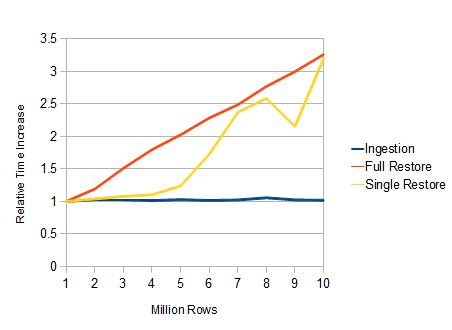
\includegraphics{loc.jpg}
\caption{Small Benchmark on a private machine}
\end{figure}


In this diagram, the relative time in- or decrease over the course of the benchmark  in relation to the very first segment, is displayed. The development shows a nearly constant ingestion rate, as expected. Ingesting a single segments took 124 seconds on average, resulting in a rate of 8460 rows/second or 947 kB/second. These results were unsurprising and met the expectations.\\
\\
However, the single restore behaved oddly. Later experiments indicate that the results likely were disturbed by extreme outliers. This subject will be adressed later on.\\\\
Unfortunately, Druid was not able to restore the full Analytics matrix in a single query. All such attempts ended in a time-out failure. In order to overcome this problem, we split the subscribers in 10 smaller groups, according to their Id. This step resolved the problem and we were able to obtain reasonable results.
As the graphic shows the query times increase only linearly and not exponentionally. After the 10th segment, the full restore was 3.5 times slower than after the first. These times were admissable, considering the amount of data had increased by a factor 10. 
\\[1cm]
The same benchmark was also run on Euler07. These following results were obtained. (See Figure 4)  

\begin{figure}[h]
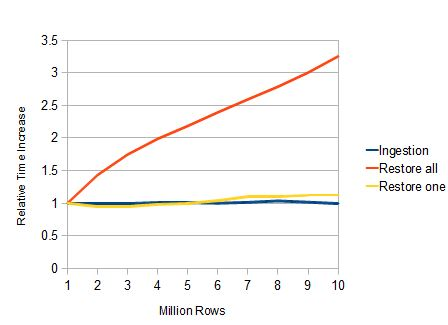
\includegraphics{meul.jpg}
\caption{Small Benchmark on the Euler07}
\end{figure}


Again, the diagram depicts the relative time in- or decreases of the 3 fields under measurement. The ingestion rate and the full restore behaved almost identical to the other benchmark, remaining constant resp. increasing up to a factor 3.5.\\
The interesting point to notice is the single record restore, which remained constant, in contrary to the previous benchmark. 


\clearpage
\subsection{Hadoop for Big Data}
In order to create a more realistic test environment, we increased the size of each data segment by a factor 10. The seperate files now contained 10'485'760 rows each and were 1.2 Gb large. In order to ingest these large datasets, we set up a single node Hadoop cluster, rather than relying on the Overlord node. Besides that the benchmark stayed pretty much the same. The following results were obtained on the same private machine as in section 4.1.

\begin{figure}[h]
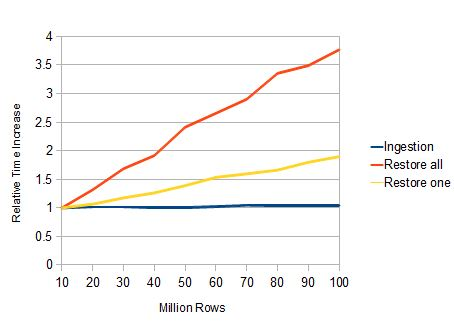
\includegraphics{loclarge.jpg}
\caption{Large Benchmark on a private machine}
\end{figure}

Once again, the ingestion rate remained more or less constant throughout the entire benchmark. It took Druid resp. Hadoop  689 seconds on average to complete the task, which results in an ingestion rate of 15'200 rows/second or 1740 kB/second. The query times behave very similar to the small benchmark.

\clearpage
\section{Summary}
\subsection{Conclusion}
Our motivating use case comes from the telecommunications industry, where
a provider wants to be able to process and analyze the usage data of its sub-
scribers. A subscriber's usage of the provider's network generates update events,
which need to be processed and stored. Providers want to query this data in
real-time to gain insights about the subscribers' behavior.\\\\
The original goal of this thesis was to execute the before mentioned AIM-benchmark on druid. However, it soon became clear that such a comparison makes little sense, since the two system are designed for completly different purposes. Druid excels at ingestion a huge continous stream of data, while having trouble updating existing data, which is one of the core strengths of AIM.\\\\
Rather than heavily modifying the AIM benchmark, we came up with a new one, which was supposed to verify Druid's suitability as a backup store for AIM, as AIM currently lacks the ability to restore its content in case of severe failure. The obtained results indicate that this is indeed the case, as Druid's ingestion rate remained constant, and the query times increased only linearly, which is acceptable.\\\\
It remains to be seen wheter Druid and AIM are able to assert themselves in the huge field of competitive data stores. There are countless competitors, such as Impala, Cassandra or Hadoop, and it would be interesting to see how they fare in direct comparison. However, this is material for future work.

\subsection{Acknowledgements}
I'd like to thank my supervisors Lucas Braun and Renato Marroquin for their continuous support and help. They provided many meaningful suggestions and proposals. Their expertise and experience was very valuable.\\\\
I'd also like to thank Professor Kossmann for taking the time to supervise my thesis.\\\\
A special thanks thanks goes to my parents for keeping me motivated and for revising this thesis.

\clearpage

\begin{thebibliography}{1}
\bibitem {druid} Fangjin Yang, Eric Tschetter, Xavier Léauté, Nelson Ray, Gian Merlino, Deep Ganguli.
{\em Druid. A Real-time Analytical Data Store}, 2014

\bibitem{aim} Lucas Braun, Thomas Etter, Georgios Gasparis,
Martin Kaufmann, Donald Kossmann, Daniel Widmer, Aharon Avitzur, Anthony Iliopoulos, Eliezer Levy, Ning Liang.
{\em Analytics in Motion. High Performance Event-Processing AND Real-Time Analytics in the Same Database}, 2015

\bibitem{druidon}
Metamarkets Inc. {\em Druid.} http://druid.io/, 2014. [Online; accessed July 2015].

\bibitem{hadoop}Apache Foundation. {\em Hadoop.} http://hadoop.apache.org/, 2013. [Online; accessed July 2015].

\bibitem{zoo}Apache Foundation. {\em Zookeeper.} http://zookeeper.apache.org/, 2014. [Online; accessed July 2015].


\end{thebibliography}

\end{document}